\documentclass[14pt, a4paper]{extarticle}

\usepackage[margin=1in]{geometry}
\usepackage{graphicx}
\usepackage{enumitem}
\usepackage{multicol}
\usepackage{fancyhdr}
\usepackage{amsfonts}
\usepackage{amssymb}
\usepackage{listings}
\usepackage{float}
\usepackage{wrapfig}

\usepackage{gvv-book}
\usepackage{gvv}

\graphicspath{ {figs/} }

\pagestyle{fancy}
\fancyhf{} 
\fancyhead[L]{2021}
\fancyhead[R]{PH}
\fancyfoot[L]{PH}
\fancyfoot[R]{\thepage/27}
\renewcommand{\headrulewidth}{0.4pt}
\renewcommand{\footrulewidth}{0.4pt}

\let\oldvec\vec
\renewcommand{\vec}[1]{\overrightarrow{#1}}
\newcommand{\myvec}[1]{\begin{bmatrix} #1 \end{bmatrix}}

\begin{document}

\section*{General Aptitude (GA)}
\textbf{Q.1 – Q.5 Multiple Choice Question (MCQ), carry ONE mark each (for each wrong answer: – 1/3).}

\begin{enumerate}[label=\textbf{Q.\arabic*}]

\item
\begin{enumerate}[(i)]
    \item Arun and Aparna are here.
    \item Arun and Aparna is here.
    \item Arun's families is here.
    \item Arun's family is here.
\end{enumerate}
Which of the above sentences are grammatically CORRECT?
\begin{enumerate}
\begin{multicols}{4}
\item (i) and (ii)
\item (i) and (iv)
\item (ii) and (iv)
\item (iii) and (iv)
\end{multicols}
\end{enumerate}

\item 
\begin{figure}[H]
\centering
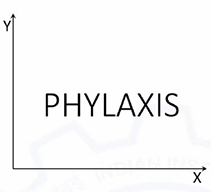
\includegraphics[width=0.4\textwidth]{figs/q2fig21.png}
\caption{text in graph}
\label{fig:q2_original}
\end{figure}
The mirror image of the above text about the X-axis is
\begin{enumerate}
\item 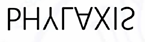
\includegraphics[width=0.5\textwidth]{figs/q2figA21.png}
\item 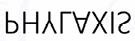
\includegraphics[width=0.5\textwidth]{figs/q2figb21.png}
\item 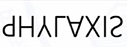
\includegraphics[width=0.5\textwidth]{figs/q2figc21.png}
\item 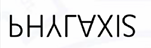
\includegraphics[width=0.5\textwidth]{figs/q2figd21.png}
\end{enumerate}
\hfill \textbf{(GATE PH 2021)}

\item Two identical cube shaped dice each with faces numbered 1 to 6 are rolled simultaneously. The probability that an even number is rolled out on each dice is:
\begin{enumerate}
\begin{multicols}{4}
\item $\frac{1}{36}$
\item $\frac{1}{12}$
\item $\frac{1}{8}$
\item $\frac{1}{4}$
\end{multicols}
\end{enumerate}
\hfill \textbf{(GATE PH 2021)}

\item $\oplus$ and $\odot$ are two operators on numbers $p$ and $q$ such that $p \odot q = p-q$, and $p \oplus q = p \times q$. Then, $(9 \odot (6 \oplus 7)) \odot (7 \oplus (6 \odot 5)) = $
\begin{enumerate}
\begin{multicols}{4}
\item 40
\item -26
\item -33
\item -40
\end{multicols}
\end{enumerate}
\hfill \textbf{(GATE PH 2021)}

\item Four persons P, Q, R and S are to be seated in a row. R should not be seated at the second position from the left end of the row. The number of distinct seating arrangements possible is:
\begin{enumerate}
\begin{multicols}{4}
\item 6
\item 9
\item 18
\item 24
\end{multicols}
\end{enumerate}
\hfill \textbf{(GATE PH 2021)}

\textbf{Q. 6 – Q. 10 Multiple Choice Question (MCQ), carry TWO marks each (for each wrong answer: – 2/3).}

\item On a planar field, you travelled 3 units East from a point O. Next you travelled 4 units South to arrive at point P. Then you travelled from P in the North-East direction such that you arrive at a point that is 6 units East of point O. Next, you travelled in the North-West direction, so that you arrive at point Q that is 8 units North of point P.
The distance of point Q to point O, in the same units, should be \underline{\hspace{3cm}}.
\begin{enumerate}
\begin{multicols}{4}
\item 3
\item 4
\item 5
\item 6
\end{multicols}
\end{enumerate}
\hfill \textbf{(GATE PH 2021)}

\item 
\begin{quote}
The author said, “Musicians rehearse before their concerts. Actors rehearse their roles before the opening of a new play. On the other hand, I find it strange that many public speakers think they can just walk on to the stage and start speaking. In my opinion, it is no less important for public speakers to rehearse their talks.”
\end{quote}
Based on the above passage, which one of the following is TRUE?
\begin{enumerate}
\item The author is of the opinion that rehearsing is important for musicians, actors and public speakers.
\item The author is of the opinion that rehearsing is less important for public speakers than for musicians and actors.
\item The author is of the opinion that rehearsing is more important only for musicians than public speakers.
\item The author is of the opinion that rehearsing is more important for actors than musicians.
\end{enumerate}
\hfill \textbf{(GATE PH 2021)}

\item
\begin{enumerate}
    \item Some football players play cricket.
    \item All cricket players play hockey.
\end{enumerate}
Among the options given below, the statement that logically follows from the two statements 1 and 2 above, is:
\begin{enumerate}
\item No football players play hockey.
\item Some football players play hockey.
\item All football players play hockey.
\item All hockey players play football.
\end{enumerate}
\hfill \textbf{(GATE PH 2021)}

\item 
\begin{figure}[H]
\centering
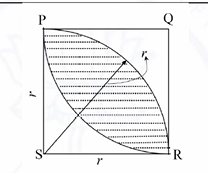
\includegraphics[width=0.3\textwidth]{figs/q9fig21.png}
\caption{square PQRS}
\label{fig:q9}
\end{figure}
In the figure shown above, PQRS is a square. The shaded portion is formed by the intersection of sectors of circles with radius equal to the side of the square and centers at S and Q.
The probability that any point picked randomly within the square falls in the shaded area is \underline{\hspace{3cm}}.
\begin{enumerate}
\begin{multicols}{4}
\item $4 - \frac{\pi}{2}$
\item $\frac{1}{2}$
\item $\frac{\pi}{2} - 1$
\item $\frac{\pi}{4}$
\end{multicols}
\end{enumerate}
\hfill \textbf{(GATE PH 2021)}

\item In an equilateral triangle PQR, side PQ is divided into four equal parts, side QR is divided into six equal parts and side PR is divided into eight equal parts. The length of each subdivided part in cm is an integer.
The minimum area of the triangle PQR possible, in cm$^2$, is
\begin{enumerate}
\begin{multicols}{4}
\item 18
\item 24
\item $48\sqrt{3}$
\item $144\sqrt{3}$
\end{multicols}
\end{enumerate}
\hfill \textbf{(GATE PH 2021)}

\section*{Physics (PH)}
\textbf{Q.1 – Q.9 Multiple Choice Question (MCQ), carry ONE mark each (for each wrong answer: – 1/3).}

\begin{enumerate}[label=\textbf{Q.\arabic*}]

\item Choose the graph that best describes the variation of dielectric constant ($\epsilon_r$) with temperature ($T$) in a ferroelectric material. ($T_C$ is the Curie temperature)
\begin{enumerate}
    \item 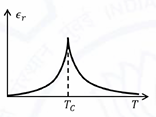
\includegraphics[width=0.4\textwidth]{figs/q11fig21.png}
    \item 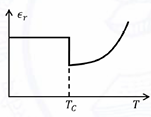
\includegraphics[width=0.4\textwidth]{figs/q11figb21.png}
    \item 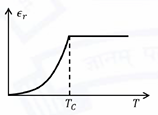
\includegraphics[width=0.4\textwidth]{figs/q11figc21.png}
    \item 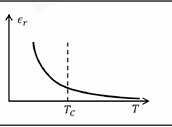
\includegraphics[width=0.4\textwidth]{figs/q11figd21.png}
\end{enumerate}
\hfill \textbf{(GATE PH 2021)}


\item A matter wave is represented by the wave function
\begin{align*}
 \Psi(x, y, z, t) = A e^{i(4x+3y+5z-10\pi t)} 
 \end{align*}
where A is a constant. The unit vector representing the direction of propagation of this matter wave is
\begin{enumerate}
\item $\frac{4}{5\sqrt{2}}\hat{x} + \frac{3}{5\sqrt{2}}\hat{y} + \frac{1}{\sqrt{2}}\hat{z}$
\item $\frac{3}{5\sqrt{2}}\hat{x} + \frac{4}{5\sqrt{2}}\hat{y} + \frac{1}{5\sqrt{2}}\hat{z}$
\item $\frac{1}{5\sqrt{2}}\hat{x} + \frac{3}{5\sqrt{2}}\hat{y} + \frac{1}{\sqrt{2}}\hat{z}$
\item $\frac{1}{\sqrt{2}}\hat{x} + \frac{4}{5\sqrt{2}}\hat{y} + \frac{3}{5\sqrt{2}}\hat{z}$
\end{enumerate}
\hfill \textbf{(GATE PH 2021)}

\item As shown in the figure, X-ray diffraction pattern is obtained from a diatomic chain of atoms P and Q. The diffraction condition is given by $a \cos \theta = n\lambda$, where $n$ is the order of the diffraction peak. Here, $a$ is the lattice constant and $\lambda$ is the wavelength of the X-rays. Assume that atomic form factors and resolution of the instrument do not depend on $\theta$. Then, the intensity of the diffraction peaks is
\begin{figure}[H]
\centering
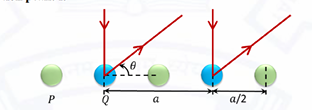
\includegraphics[width=0.6\textwidth]{figs/q13fig21.png}
\caption{X-ray diffraction pattern}
\end{figure}
\begin{enumerate}
\item lower for even values of $n$, when compared to odd values of $n$
\item lower for odd values of $n$, when compared to even values of $n$
\item zero for odd values of $n$
\item zero for even values of $n$
\end{enumerate}
\hfill \textbf{(GATE PH 2021)}

\item As shown in the figure, two metal-semiconductor junctions are formed between an n-type semiconductor $S$ and metal $M$. The work functions of $S$ and $M$ are $\phi_S$ and $\phi_M$, respectively with $\phi_M > \phi_S$.
\begin{figure}[H]
\centering
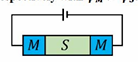
\includegraphics[width=0.3\textwidth]{figs/q4fig21.png}
\caption{wo metal-semiconductor junctions formed
between an n-type semiconductor S and metal M.}
\end{figure}
The $I-V$ characteristics (on linear scale) of the junctions is best represented by
\begin{enumerate}
\item 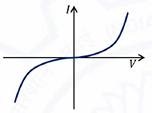
\includegraphics[width=0.4\textwidth]{figs/q14figa21.png}
\item 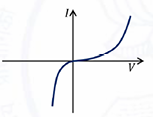
\includegraphics[width=0.4\textwidth]{figs/q14figb21.png}
\item 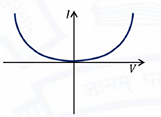
\includegraphics[width=0.4\textwidth]{figs/q14figc21.png}
\item 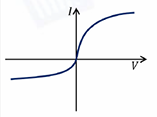
\includegraphics[width=0.4\textwidth]{figs/q14figd21.png}
\end{enumerate}
\hfill \textbf{(GATE PH 2021)}

\item Consider a tiny current loop driven by a sinusoidal alternating current. If the surface integral of its time-averaged Poynting vector is constant, then the magnitude of the time-averaged magnetic field intensity, at any arbitrary position, $\vec{r}$, is proportional to
\begin{enumerate}
\begin{multicols}{4}
\item $\frac{1}{r^3}$
\item $\frac{1}{r^2}$
\item $\frac{1}{r}$
\item $r$
\end{multicols}
\end{enumerate}
\hfill \textbf{(GATE PH 2021)}


\item Consider a solenoid of length $L$ and radius $R$, where $R \ll L$. A steady-current flows through the solenoid. The magnetic field is uniform inside the solenoid and zero outside.
\begin{figure}[H]
\centering
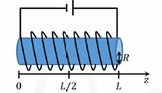
\includegraphics[width=0.3\textwidth]{figs/q16fig21.png}
\caption{a solenoid of length L and radius R}
\end{figure}
Among the given options, choose the one that best represents the variation in the magnitude of the vector potential, $(0, A_\phi, 0)$ at $z = L/2$, as a function of the radial distance ($r$) in cylindrical coordinates. \\
\textbf{Useful information:} The curl of a vector $\mathbf{F}$, in cylindrical coordinates is
$$ \nabla \times \mathbf{F}(r, \phi, z) = \hat{r}\left[\frac{1}{r}\frac{\partial F_z}{\partial \phi} - \frac{\partial F_\phi}{\partial z}\right] + \hat{\phi}\left[\frac{\partial F_r}{\partial z} - \frac{\partial F_z}{\partial r}\right] + \hat{z}\frac{1}{r}\left[\frac{\partial (rF_\phi)}{\partial r} - \frac{\partial F_r}{\partial \phi}\right] $$
\begin{enumerate}
\item 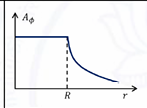
\includegraphics[width=0.5\textwidth]{figs/q16figa21.png}
\item 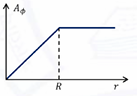
\includegraphics[width=0.5\textwidth]{figs/q16figb21.png}
\item 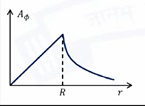
\includegraphics[width=0.5\textwidth]{figs/q16figc21.png}
\item 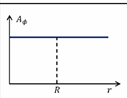
\includegraphics[width=0.5\textwidth]{figs/q16figd21.png}
\end{enumerate}
\hfill \textbf{(GATE PH 2021)}

\item Assume that $^{13}$N (Z = 7) undergoes first forbidden $\beta^+$ decay from its ground state with spin-parity $J_i^{\pi}$, to a final state $J_f^{\pi}$. The possible values for $J_i^{\pi}$ and $J_f^{\pi}$, respectively, are
\begin{enumerate}
\begin{multicols}{4}
\item $\frac{1}{2}^-, \frac{5}{2}^+$
\item $\frac{1}{2}^+, \frac{5}{2}^+$
\item $\frac{1}{2}^-, \frac{1}{2}^-$
\item $\frac{1}{2}^+, \frac{1}{2}^-$
\end{multicols}
\end{enumerate}
\hfill \textbf{(GATE PH 2021)}

\item In an experiment, it is seen that an electric-dipole (E1) transition can connect an initial nuclear state of spin-parity $J_i^{\pi} = 2^+$ to a final state $J_f^{\pi}$. All possible values of $J_f^{\pi}$ are
\begin{enumerate}
\begin{multicols}{4}
\item $1^+, 2^+$
\item $1^+, 2^+, 3^+$
\item $1^-, 2^-$
\item $1^-, 2^-, 3^-$
\end{multicols}
\end{enumerate}
\hfill \textbf{(GATE PH 2021)}

\item Choose the correct statement from the following.
\begin{enumerate}
\item Silicon is a direct band gap semiconductor.
\item Conductivity of metals decreases with increase in temperature.
\item Conductivity of semiconductors decreases with increase in temperature.
\item Gallium Arsenide is an indirect band gap semiconductor.
\end{enumerate}
\hfill \textbf{(GATE PH 2021)}

\textbf{Q.10 – Q.16 Multiple Select Question (MSQ), carry ONE mark each (no negative marks).}

\item A two-dimensional square lattice has lattice constant $a$. $k$ represents the wavevector in reciprocal space. The coordinates ($k_x, k_y$) of reciprocal space where band gap(s) can occur, are
\begin{enumerate}
\begin{multicols}{4}
\item $(0, 0)$
\item $\left(\pm \frac{\pi}{a}, \pm \frac{\pi}{a}\right)$
\item $\left(\pm \frac{\pi}{a}, \pm \frac{\pi}{1.3a}\right)$
\item $\left(\pm \frac{\pi}{3a}, \pm \frac{\pi}{a}\right)$
\end{multicols}
\end{enumerate}
\hfill \textbf{(GATE PH 2021)}

\item As shown in the figure, an electromagnetic wave with intensity $I_I$ is incident at the interface of two media having refractive indices $n_1 = 1$ and $n_2 = \sqrt{3}$. The wave is reflected with intensity $I_R$ and transmitted with intensity $I_T$. Permeability of each medium is the same. (Reflection coefficient $R = I_R/I_I$ and Transmission coefficient $T = I_T/I_I$).
\begin{figure}[H]
\centering
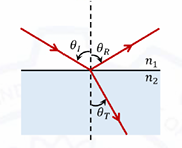
\includegraphics[width=0.35\textwidth]{figs/q21fig21.png}
\caption{electromagnetic wave with intensity II is in-
cident at the interface of two media}
\end{figure}
Choose the correct statement(s).
\begin{enumerate}
\item $R=0$ if $\theta_I = 0^{\circ}$ and polarization of incident light is parallel to the plane of incidence.
\item $T=1$ if $\theta_I = 60^{\circ}$ and polarization of incident light is parallel to the plane of incidence.
\item $R=0$ if $\theta_I = 60^{\circ}$ and polarization of incident light is perpendicular to the plane of incidence.
\item $T=1$ if $\theta_I = 60^{\circ}$ and polarization of incident light is perpendicular to the plane of incidence.
\end{enumerate}
\hfill \textbf{(GATE PH 2021)}

\item A material is placed in a magnetic field intensity $H$. As a result, bound current density $J_b$ is induced and magnetization of the material is $M$. The magnetic flux density is $B$. Choose the correct option(s) valid at the \textit{surface} of the material.
\begin{enumerate}
\begin{multicols}{4}
\item $\nabla \cdot M = 0$
\item $\nabla \cdot B = 0$
\item $\nabla \cdot H = 0$
\item $\nabla \cdot J_b = 0$
\end{multicols}
\end{enumerate}
\hfill \textbf{(GATE PH 2021)}

\item For a finite system of Fermions where the density of states increases with energy, the chemical potential
\begin{enumerate}
\item decreases with temperature
\item increases with temperature
\item does not vary with temperature
\item corresponds to the energy where the occupation probability is 0.5
\end{enumerate}
\hfill \textbf{(GATE PH 2021)}

\item Among the term symbols $^4S_1$, $^2D_{7/2}$, $^3S_1$ and $^2D_{5/2}$ choose the option(s) possible in the LS coupling notation.
\begin{enumerate}
\begin{multicols}{4}
\item $^4S_1$
\item $^2D_{7/2}$
\item $^3S_1$
\item $^2D_{5/2}$
\end{multicols}
\end{enumerate}
\hfill \textbf{(GATE PH 2021)}

\item To sustain lasing action in a three-level laser as shown in the figure, necessary condition(s) is(are)
\begin{figure}[H]
\centering
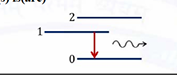
\includegraphics[width=0.3\textwidth]{figs/q25fig21.png}
\caption{three-level laser}
\end{figure}
\begin{enumerate}
\item lifetime of the energy level 1 should be greater than that of energy level 2
\item population of the particles in level 1 should be greater than that of level 0
\item lifetime of the energy level 2 should be greater than that of energy level 0
\item population of the particles in level 2 should be greater than that of level 1
\end{enumerate}
\hfill \textbf{(GATE PH 2021)}

\item If $y_n(x)$ is a solution of the differential equation $y'' - 2xy' + 2ny = 0$ where $n$ is an integer and the prime (') denotes differentiation with respect to $x$, then acceptable plot(s) of $\psi_n(x) = e^{-x^2/2} y_n(x)$, is(are)
\begin{enumerate}
\item 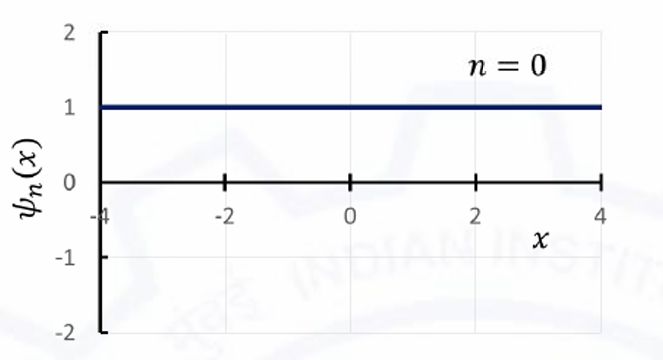
\includegraphics[width=0.5\textwidth]{figs/q26figa21.png}
\item 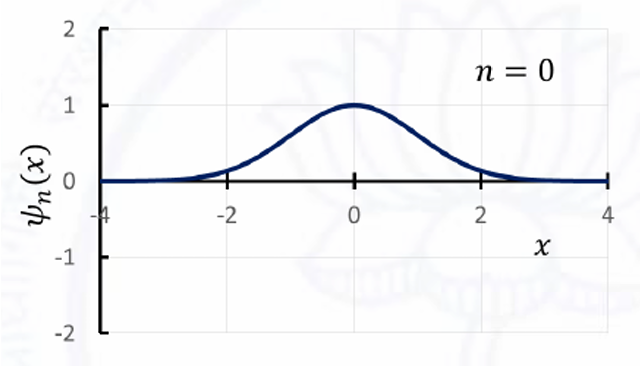
\includegraphics[width=0.5\textwidth]{figs/q26figb21.png}
\item 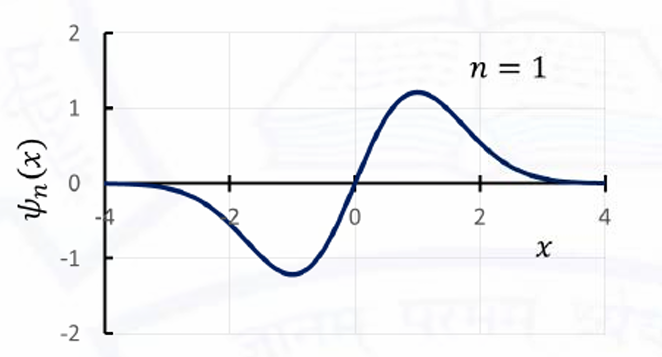
\includegraphics[width=0.5\textwidth]{figs/q26figc21.png}
\item 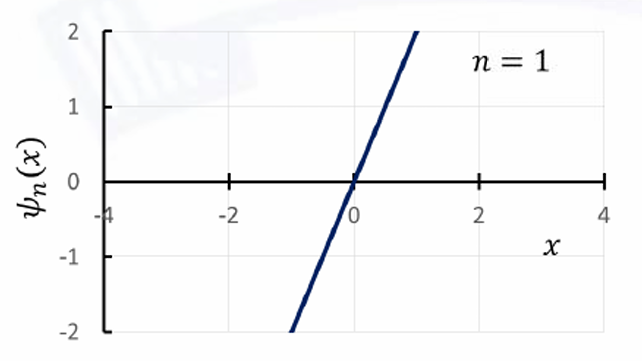
\includegraphics[width=0.5\textwidth]{figs/q26figd21.png}
\end{enumerate}
\hfill \textbf{(GATE PH 2021)}

\textbf{Q.17 – Q.25 Numerical Answer Type (NAT), carry ONE mark each (no negative marks).}

\item The donor concentration in a sample of n-type silicon is increased by a factor of 100. Assuming the sample to be non-degenerate, the shift in the Fermi level (in meV) at 300 K (rounded off to the nearest integer) is \underline{\hspace{3cm}}.
(Given: $k_B T = 25$ meV at 300 K)
\hfill \textbf{(GATE PH 2021)}

\item Two observers $O$ and $O'$ observe two events $P$ and $Q$. The observers have a constant relative speed of 0.5c. In the units, where the speed of light, c, is taken as unity, the observer $O$ obtained the following coordinates:
\begin{itemize}
    \item[] Event P: x=5, y=3, z=5, t=3
    \item[] Event Q: x=5, y=1, z=3, t=5
\end{itemize}
The length of the space-time interval between these two events, as measured by $O'$, is L. The value of $|L|$ (in integer) is \underline{\hspace{3cm}}.
\hfill \textbf{(GATE PH 2021)}

\item A light source having its intensity peak at the wavelength 289.8 nm is calibrated as 10,000 K which is the temperature of an equivalent black body radiation. Considering the same calibration, the temperature of light source (in K) having its intensity peak at the wavelength 579.6 nm (rounded off to the nearest integer) is \underline{\hspace{3cm}}.
\hfill \textbf{(GATE PH 2021)}

\item A hoop of mass $M$ and radius $R$ rolls without slipping along a straight line on a horizontal surface as shown in the figure. A point mass $m$ slides without friction along the inner surface of the hoop, performing small oscillations about the mean position. The number of degrees of freedom of the system (in integer) is \underline{\hspace{3cm}}.
\begin{figure}[H]
\centering
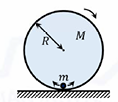
\includegraphics[width=0.3\textwidth]{figs/q30fig21.png}
\caption{hoop of mass M and radius R}
\end{figure}
\hfill \textbf{(GATE PH 2021)}

\item Three non-interacting bosonic particles of mass $m$ each, are in a one-dimensional infinite potential well of width $a$. The energy of the third excited state of the system is $x \times \frac{h^2\pi^2}{ma^2}$. The value of $x$ (in integer) is \underline{\hspace{3cm}}.
\hfill \textbf{(GATE PH 2021)}

\item The spacing between two consecutive S-branch lines of the rotational Raman spectra of hydrogen gas is 243.2 cm$^{-1}$. After excitation with a laser of wavelength 514.5 nm, the Stoke's line appeared at 17611.4 cm$^{-1}$ for a particular energy level. The wavenumber (rounded off to the nearest integer), in cm$^{-1}$, at which Stoke's line will appear for the next higher energy level is \underline{\hspace{3cm}}.
\hfill \textbf{(GATE PH 2021)}

\item The transition line, as shown in the figure, arises between $^2D_{3/2}$ and $^2P_{1/2}$ states without any external magnetic field. The number of lines that will appear in the presence of a weak magnetic field (in integer) is \underline{\hspace{3cm}}.
\begin{figure}[H]
\centering
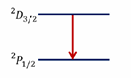
\includegraphics[width=0.3\textwidth]{figs/q33fig21.png}
\caption{transition line}
\end{figure}
\hfill \textbf{(GATE PH 2021)}

\item Consider the atomic system as shown in the figure, where the Einstein $A$ coefficients for spontaneous emission for the levels are $A_{2\to1} = 2 \times 10^7$ s$^{-1}$ and $A_{1\to0} = 10^8$ s$^{-1}$. If $10^{14}$ atoms/cm$^3$ are excited from level 0 to level 2 and a steady state population in level 2 is achieved, then the steady state population at level 1 will be $x \times 10^{13}$ cm$^{-3}$. The value of $x$ (in integer) is \underline{\hspace{3cm}}.
\begin{figure}[H]
\centering
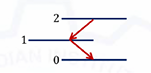
\includegraphics[width=0.3\textwidth]{figs/q34fig21.png}
\caption{atomic system figure}
\end{figure}
\hfill \textbf{(GATE PH 2021)}

\item If $\vec{a}$ and $\vec{b}$ are constant vectors, $\vec{r}$ and $\vec{p}$ are generalized positions and conjugate momenta, respectively, then for the transformation $Q = \vec{a} \cdot \vec{p}$ and $P = \vec{b} \cdot \vec{r}$ to be canonical, the value of $\vec{a} \cdot \vec{b}$ (in integer) is \underline{\hspace{3cm}}.
\hfill \textbf{(GATE PH 2021)}

\textbf{Q.26 – Q.41 Multiple Choice Question (MCQ), carry TWO mark each (for each wrong answer: – 2/3).}

\item
\begin{figure}[H]
\centering
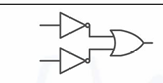
\includegraphics[width=0.3\textwidth]{figs/q36fig21.png}
\caption{Logic gate combination.}
\label{fig:q26ph}
\end{figure}
The above combination of logic gates represents the operation
\begin{enumerate}
\begin{multicols}{4}
\item OR
\item NAND
\item AND
\item NOR
\end{multicols}
\end{enumerate}
\hfill \textbf{(GATE PH 2021)}

\item In a semiconductor, the ratio of the effective mass of hole to electron is 2:11 and the ratio of average relaxation time for hole to electron is 1:2. The ratio of the mobility of the hole to electron is
\begin{enumerate}
\begin{multicols}{4}
\item 4:9
\item 4:11
\item 9:4
\item 11:4
\end{multicols}
\end{enumerate}
\hfill \textbf{(GATE PH 2021)}

\item Consider a spin $S = \hbar/2$ particle in the state $|\phi\rangle = \frac{1}{3}\begin{bmatrix} 2+i \\ 2 \end{bmatrix}$. The probability that a measurement finds the state with $S_x = +\hbar/2$ is
\begin{enumerate}
\begin{multicols}{4}
\item 5/18
\item 11/18
\item 15/18
\item 17/18
\end{multicols}
\end{enumerate}
\hfill \textbf{(GATE PH 2021)}

\item An electromagnetic wave having electric field $E = 8 \cos(kz - \omega t) \hat{y}$ V cm$^{-1}$ is incident at $90^{\circ}$(normal incidence) on a square slab from vacuum (with refractive index $n_0 = 1.0$) as shown in the figure. The slab is composed of two different materials with refractive indices $n_1=2.2$ and $n_2=1.1$. Assume that the permeability of each medium is the same. After passing through the slab for the first time, the electric field amplitude, in V cm$^{-1}$, of the electromagnetic wave, which emerges from the slab in region 2, is closest to
\begin{figure}[H]
\centering
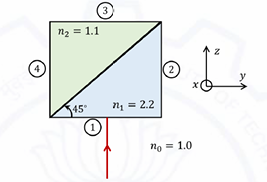
\includegraphics[width=0.4\textwidth]{figs/q39fig21.png}
\caption{EM wave incident on a composite slab.}
\label{fig:q29ph}
\end{figure}
\begin{enumerate}
\begin{multicols}{4}
\item $\frac{11}{1.6}$
\item $\frac{11}{3.2}$
\item $\frac{11}{13.8}$
\item $\frac{11}{25.6}$
\end{multicols}
\end{enumerate}
\hfill \textbf{(GATE PH 2021)}

\item Consider a point charge $+Q$ of mass $m$ suspended by a massless, inextensible string of length $l$ in free space (permittivity $\epsilon_0$) as shown in the figure. It is placed at a height $d$ ($d > l$) over an infinitely large, grounded conducting plane. The gravitational potential energy is assumed to be zero at the position of the conducting plane and is positive above the plane.
\begin{figure}[H]
\centering
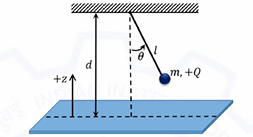
\includegraphics[width=0.4\textwidth]{figs/q40fig21.png}
\caption{Charged pendulum above a conducting plane.}
\label{fig:q30ph}
\end{figure}
If $\theta$ represents the angular position and $p_{\theta}$ its corresponding canonical momentum, then the correct Hamiltonian of the system is
\begin{enumerate}
\item $\frac{p_{\theta}^2}{2ml^2} - \frac{Q^2}{16\pi\epsilon_0(d-l\cos\theta)} - mg(d-l\cos\theta)$
\item $\frac{p_{\theta}^2}{2ml^2} - \frac{Q^2}{8\pi\epsilon_0(d-l\cos\theta)} + mg(d-l\cos\theta)$
\item $\frac{p_{\theta}^2}{2ml^2} - \frac{Q^2}{8\pi\epsilon_0(d-l\cos\theta)} - mg(d-l\cos\theta)$
\item $\frac{p_{\theta}^2}{2ml^2} - \frac{Q^2}{16\pi\epsilon_0(d-l\cos\theta)} + mg(d-l\cos\theta)$
\end{enumerate}
\hfill \textbf{(GATE PH 2021)}

\item Consider two concentric conducting spherical shells as shown in the figure. The inner shell has a radius $a$ and carries a charge $+Q$. The outer shell has a radius $b$ and carries a charge $-Q$. The empty space between them is half-filled by a hemispherical shell of a dielectric having permittivity $\epsilon_1$. The remaining space between the shells is filled with air having the permittivity $\epsilon_0$.
\begin{figure}[H]
\centering
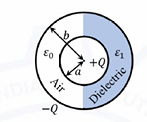
\includegraphics[width=0.3\textwidth]{figs/q41fig21.png}
\caption{Concentric spherical shells with dielectric and air.}
\label{fig:q31ph}
\end{figure}
The electric field at a radial distance $r$ from the center and between the shells ($a < r < b$) is
\begin{enumerate}
\item $\frac{Q}{2\pi(\epsilon_0+\epsilon_1)r^2}\hat{r}$ everywhere
\item $\frac{Q}{4\pi\epsilon_0 r^2}\hat{r}$ on the air side and $\frac{Q}{4\pi\epsilon_1 r^2}\hat{r}$ on the dielectric side
\item $\frac{Q}{2\pi\epsilon_0 r^2}\hat{r}$ on the air side and $\frac{Q}{2\pi\epsilon_1 r^2}\hat{r}$ on the dielectric side
\item $\frac{Q}{4\pi(\epsilon_0+\epsilon_1)r^2}\hat{r}$ everywhere
\end{enumerate}
\hfill \textbf{(GATE PH 2021)}

\item
\begin{figure}[H]
\centering
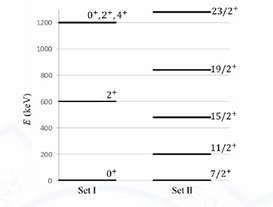
\includegraphics[width=0.6\textwidth]{figs/q42fig21.png}
\caption{Nuclear energy level schemes for two nuclei.}
\label{fig:q32ph}
\end{figure}
For the given sets of energy levels of nuclei X and Y whose mass numbers are odd and even, respectively, choose the best suited interpretation.
\begin{enumerate}
\item Set I: Rotational band of X \\ Set II: Vibrational band of Y
\item Set I: Rotational band of Y \\ Set II: Vibrational band of X
\item Set I: Vibrational band of X \\ Set II: Rotational band of Y
\item Set I: Vibrational band of Y \\ Set II: Rotational band of X
\end{enumerate}
\hfill \textbf{(GATE PH 2021)}

\item Consider a system of three distinguishable particles, each having spin $S = 1/2$ such that $S_z = \pm 1/2$ with corresponding magnetic moments $\mu_z = \pm \mu$. When the system is placed in an external magnetic field $H$ pointing along the z-axis, the total energy of the system is $\mu H$. Let $x$ be the state where the first spin has $S_z = 1/2$. The probability of having the state $x$ and the mean magnetic moment (in the $+z$ direction) of the system in state $x$ are
\begin{enumerate}
\begin{multicols}{4}
\item $\frac{1}{3}, -\frac{1}{3}\mu$
\item $\frac{1}{3}, \frac{2}{3}\mu$
\item $\frac{2}{3}, -\frac{2}{3}\mu$
\item $\frac{2}{3}, \frac{1}{3}\mu$
\end{multicols}
\end{enumerate}
\hfill \textbf{(GATE PH 2021)}

\item Consider a particle in a one-dimensional infinite potential well with its walls at $x=0$ and $x=L$. The system is perturbed as shown in the figure.
\begin{figure}[H]
\centering
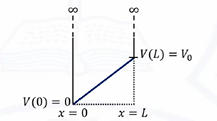
\includegraphics[width=0.3\textwidth]{figs/q44fig21.png}
\caption{Perturbation potential in an infinite well.}
\label{fig:q34ph}
\end{figure}
The first order correction to the energy eigenvalue is
\begin{enumerate}
\begin{multicols}{4}
\item $\frac{V_0}{4}$
\item $\frac{V_0}{3}$
\item $\frac{V_0}{2}$
\item $\frac{V_0}{5}$
\end{multicols}
\end{enumerate}
\hfill \textbf{(GATE PH 2021)}

\item Consider a state described by $\psi(x,t) = \psi_2(x,t) + \psi_4(x,t)$, where $\psi_2(x,t)$ and $\psi_4(x,t)$ are respectively the second and fourth normalized harmonic oscillator wave functions and $\omega$ is the angular frequency of the harmonic oscillator. The wave function $\psi(x,t=0)$ will be orthogonal to $\psi(x,t)$ at time $t$ equal to
\begin{enumerate}
\begin{multicols}{4}
\item $\frac{\pi}{2\omega}$
\item $\frac{\pi}{\omega}$
\item $\frac{\pi}{4\omega}$
\item $\frac{\pi}{6\omega}$
\end{multicols}
\end{enumerate}
\hfill \textbf{(GATE PH 2021)}

\item Consider a single one-dimensional harmonic oscillator of angular frequency $\omega$, in equilibrium at temperature $T = (k_B \beta)^{-1}$. The states of the harmonic oscillator are all non-degenerate having energy $E_n = \left(n+\frac{1}{2}\right)\hbar\omega$ with equal probability, where n is the quantum number. The Helmholtz free energy of the oscillator is
\begin{enumerate}
\item $\frac{\hbar\omega}{2} + \beta^{-1}\ln[1-\exp(\beta\hbar\omega)]$
\item $\frac{\hbar\omega}{2} + \beta^{-1}\ln[1-\exp(-\beta\hbar\omega)]$
\item $\frac{\hbar\omega}{2} + \beta^{-1}\ln[1+\exp(-\beta\hbar\omega)]$
\item $\beta^{-1}\ln[1-\exp(-\beta\hbar\omega)]$
\end{enumerate}
\hfill \textbf{(GATE PH 2021)}

\item A system of two atoms can be in three quantum states having energies $0, \epsilon$ and $2\epsilon$. The system is in equilibrium at temperature $T = (k_B\beta)^{-1}$. Match the following Statistics with the Partition function.
\begin{center}
\renewcommand{\arraystretch}{2.2}
\begin{tabular}{|p{5cm}|l|}
\hline
\textbf{Statistics} & \textbf{Partition function} \\
\hline
CD: Classical (distinguishable particles) & Z1: $e^{-\beta\epsilon} + e^{-2\beta\epsilon} + e^{-3\beta\epsilon}$ \\
\hline
CI: Classical (indistinguishable particles) & Z2: $1 + e^{-\beta\epsilon} + e^{-2\beta\epsilon} + e^{-3\beta\epsilon} + e^{-4\beta\epsilon}$ \\
\hline
FD: Fermi-Dirac & Z3: $1 + 2e^{-\beta\epsilon} + 3e^{-2\beta\epsilon} + 2e^{-3\beta\epsilon} + e^{-4\beta\epsilon}$ \\
\hline
BE: Bose-Einstein & Z4: $\frac{1}{2} + e^{-\beta\epsilon} + \frac{3}{2}e^{-2\beta\epsilon} + e^{-3\beta\epsilon} + \frac{1}{2}e^{-4\beta\epsilon}$ \\
\hline
\end{tabular}
\end{center}
\begin{enumerate}
\item CD:Z1, CI:Z2, FD:Z3, BE:Z4
\item CD:Z2, CI:Z3, FD:Z4, BE:Z1
\item CD:Z3, CI:Z4, FD:Z1, BE:Z2
\item CD:Z4, CI:Z1, FD:Z2, BE:Z3
\end{enumerate}
\hfill \textbf{(GATE PH 2021)}

\item The free energy of a ferromagnet is given by $F = F_0 + a_0(T-T_C)M^2 + bM^4$, where $F_0$, $a_0$, and $b$ are positive constants, $M$ is the magnetization, $T$ is the temperature, and $T_C$ is the Curie temperature. The relation between $M^2$ and $T$ is best depicted by
\begin{enumerate}[(A)]
\item 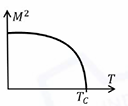
\includegraphics[width=0.4\textwidth]{figs/q48figa21.png}
\item 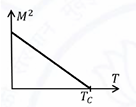
\includegraphics[width=0.4\textwidth]{figs/q48figb21.png}
\item 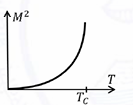
\includegraphics[width=0.4\textwidth]{figs/q48figc21.png}
\item 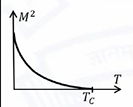
\includegraphics[width=0.4\textwidth]{figs/q48figd21.png}
\end{enumerate}
\hfill \textbf{(GATE PH 2021)}

\item Consider a spherical galaxy of total mass $M$ and radius $R$, having a uniform matter distribution. In this idealized situation, the orbital speed $v$ of a star of mass $m$ ($m \ll M$) as a function of the distance $r$ from the galactic centre is best described by ($G$ is the universal gravitational constant)
\begin{enumerate}[(A)]
\item 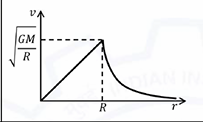
\includegraphics[width=0.5\textwidth]{figs/q49figa21.png}
\item 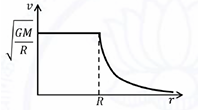
\includegraphics[width=0.5\textwidth]{figs/q49figb21.png}
\item 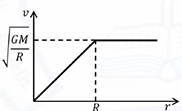
\includegraphics[width=0.5\textwidth]{figs/q49figc21.png}
\item 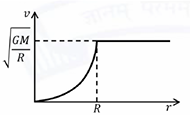
\includegraphics[width=0.5\textwidth]{figs/q49figd21.png}
\end{enumerate}
\hfill \textbf{(GATE PH 2021)}

\item Consider the potential $U(r)$ defined as

$$ U(r) = -U_0 \frac{e^{-\alpha r}}{r} $$
where $\alpha$ and $U_0$ are real constants of appropriate dimensions. According to the first Born approximation, the elastic scattering amplitude calculated with $U(r)$ for a (wave-vector) momentum transfer $q$ and $\alpha \to 0$, is proportional to \\
\textit{(Useful integral: $\int_0^{\infty} \sin(qr)e^{-\alpha r} dr = \frac{q}{\alpha^2+q^2}$)}
\begin{enumerate}
\begin{multicols}{4}
\item $q^{-2}$
\item $q^{-1}$
\item $q$
\item $q^2$
\end{multicols}
\end{enumerate}
\hfill \textbf{(GATE PH 2021)}

\item As shown in the figure, inverse magnetic susceptibility ($1/\chi$) is plotted as a function of temperature ($T$) for three different materials in paramagnetic states.
\begin{figure}[H]
\centering
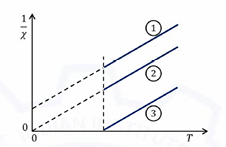
\includegraphics[width=0.5\textwidth]{figs/q51fig21.png}
\caption{Inverse magnetic susceptibility versus temperature.}
\label{fig:q41ph}
\end{figure}
(Curie temperature of ferromagnetic material=$T_C$ \\
Néel temperature of antiferromagnetic material=$T_N$) \\
Choose the correct statement from the following
\begin{enumerate}
\item Material 1 is antiferromagnetic ($T < T_N$), 2 is paramagnetic, and 3 is ferromagnetic ($T < T_C$).
\item Material 1 is paramagnetic, 2 is antiferromagnetic ($T < T_N$), and 3 is ferromagnetic ($T < T_C$).
\item Material 1 ferromagnetic ($T < T_C$), 2 is antiferromagnetic ($T < T_N$), and 3 is paramagnetic.
\item Material 1 is ferromagnetic ($T < T_C$), 2 is paramagnetic, and 3 is antiferromagnetic ($T < T_N$).
\end{enumerate}
\hfill \textbf{(GATE PH 2021)}

\textbf{Q.42 – Q.46 Multiple Select Question (MSQ), carry TWO mark each (no negative marks).}

\item A function $f(t)$ is defined only for $t \geq 0$. The Laplace transform of $f(t)$ is
$$ \mathcal{L}\{f;s\} = \int_0^{\infty} e^{-st} f(t) dt $$
whereas the Fourier transform of $f(t)$ is
$$ \mathcal{F}(\omega) = \int_0^{\infty} f(t) e^{-i\omega t} dt. $$
The correct statement(s) is(are)
\begin{enumerate}
\item The variable $s$ is always real.
\item The variable $s$ can be complex.
\item $\mathcal{L}\{f;s\}$ and $\mathcal{F}(\omega)$ can never be made connected.
\item $\mathcal{L}\{f;s\}$ and $\mathcal{F}(\omega)$ can be made connected.
\end{enumerate}
\hfill \textbf{(GATE PH 2021)}

\item $P$ and $Q$ are two Hermitian matrices and there exists a matrix $R$, which diagonalizes both of them, such that $RPR^{-1}=S_1$ and $RQR^{-1}=S_2$, where $S_1$ and $S_2$ are diagonal matrices. The correct statement(s) is(are)
\begin{enumerate}
\item All the elements of both matrices $S_1$ and $S_2$ are real.
\item The matrix $PQ$ can have complex eigenvalues.
\item The matrix $QP$ can have complex eigenvalues.
\item The matrices $P$ and $Q$ commute.
\end{enumerate}
\hfill \textbf{(GATE PH 2021)}

\item A uniform block of mass $M$ slides on a smooth horizontal bar. Another mass $m$ is connected to it by an inextensible string of length $l$ of negligible mass, and is constrained to oscillate in the X-Y plane only. Neglect the sizes of the masses. The number of degrees of freedom of the system is two and the generalized coordinates are chosen as $x$ and $\theta$, as shown in the figure.
\begin{figure}[H]
\centering
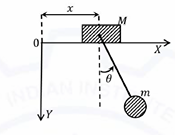
\includegraphics[width=0.4\textwidth]{figs/q54fig21.png}
\caption{A block with a pendulum attached.}
\label{fig:q44ph}
\end{figure}
If $p_x$ and $p_{\theta}$ are the generalized momenta corresponding to $x$ and $\theta$, respectively, then the correct option(s) is(are)
\begin{enumerate}
\item $p_x = (m+M)\dot{x} + ml\cos\theta\dot{\theta}$
\item $p_{\theta} = ml^2\dot{\theta} - ml\cos\theta\dot{x}$
\item $p_x$ is conserved
\item $p_{\theta}$ is conserved
\end{enumerate}
\hfill \textbf{(GATE PH 2021)}

\item The Gell-Mann – Okubo mass formula defines the mass of baryons as $M=M_0+aY+b\left[I(I+1)-\frac{1}{4}Y^2\right]$, where $M_0$, $a$ and $b$ are constants, $I$ represents the isospin and $Y$ represents the hypercharge. If the mass of $\Sigma$ hyperons is same as that of $\Lambda$ hyperons, then the correct option(s) is(are)
\begin{enumerate}
\item $M \propto I(I+1)$
\item $M \propto Y$
\item $M$ does not depend on $I$
\item $M$ does not depend on $Y$
\end{enumerate}
\hfill \textbf{(GATE PH 2021)}

\item The time derivative of a differentiable function $g(q_i, t)$ is added to a Lagrangian $L(q_i, \dot{q}_i, t)$ such that
$$ L' = L(q_i, \dot{q}_i, t) + \frac{d}{dt}g(q_i, t) $$
where $q_i, \dot{q}_i, t$ are the generalized coordinates, generalized velocities and time, respectively. Let $p_i$ be the generalized momentum and $H$ the Hamiltonian associated with $L(q_i, \dot{q}_i, t)$. If $p_i'$ and $H'$ are those associated with $L'$, then the correct option(s) is(are)
\begin{enumerate}
\item Both $L$ and $L'$ satisfy the Euler-Lagrange's equations of motion
\item $p_i' = p_i + \frac{\partial}{\partial q_i} g(q_i, t)$
\item If $p_i$ is conserved, then $p_i'$ is necessarily conserved
\item $H' = H + \frac{d}{dt}g(q_i, t)$
\end{enumerate}
\hfill \textbf{(GATE PH 2021)}

\textbf{Q.47 – Q.55 Numerical Answer Type (NAT), carry TWO mark each (no negative marks).}

\item A linear charged particle accelerator is driven by an alternating voltage source operating at 10 MHz. Assume that it is used to accelerate electrons. After a few drift-tubes, the electrons attain a velocity $2.9 \times 10^8$ m s$^{-1}$. The minimum length of each drift-tube, in m, to accelerate the electrons further (rounded off to one decimal place) is \underline{\hspace{3cm}}.
\hfill \textbf{(GATE PH 2021)}

\item The Coulomb energy component in the binding energy of a nucleus is 18.432 MeV. If the radius of the uniform and spherical charge distribution in the nucleus is 3 fm, the corresponding atomic number (rounded off to the nearest integer) is \underline{\hspace{3cm}}.
(Given: $\frac{e^2}{4\pi\epsilon_0} = 1.44$ MeV fm)
\hfill \textbf{(GATE PH 2021)}

\item For a two-nucleon system in spin singlet state, the spin is represented through the Pauli matrices $\sigma_1, \sigma_2$ for particles 1 and 2, respectively. The value of $(\sigma_1 \cdot \sigma_2)$ (in integer) is \underline{\hspace{3cm}}.
\hfill \textbf{(GATE PH 2021)}

\item A contour integral is defined as
$$ I_n = \oint_C \frac{dz}{(z-n)^2 + \pi^2} $$
where $n$ is a positive integer and $C$ is the closed contour, as shown in the figure, consisting of the line from $-100$ to $100$ and the semicircle traversed in the counter-clockwise sense.
\begin{figure}[H]
\centering
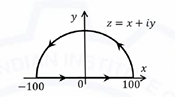
\includegraphics[width=0.4\textwidth]{figs/q60fig21.png}
\caption{Closed contour C in the complex plane.}
\label{fig:q50ph}
\end{figure}
The value of $\sum_{n=1}^{5} I_n$ (in integer) is \underline{\hspace{3cm}}.

\item The normalized radial wave function of the second excited state of hydrogen atom is
$$ R(r) = \frac{1}{\sqrt{24}} a^{-3/2} \frac{r}{a} e^{-r/2a} $$
where $a$ is the Bohr radius and $r$ is the distance from the center of the atom. The distance at which the electron is most likely to be found is $y \times a$. The value of $y$ (in integer) is \underline{\hspace{3cm}}.
\hfill \textbf{(GATE PH 2021)}

\item Consider an atomic gas with number density $n = 10^{20}$ m$^{-3}$, in the ground state at 300 K. The valence electronic configuration of atoms is $f^7$. The paramagnetic susceptibility of the gas $\chi = m \times 10^{-11}$. The value of $m$ (rounded off to two decimal places) is \underline{\hspace{3cm}}.
(Given: Magnetic permeability of free space $\mu_0 = 4\pi \times 10^{-7}$ H m$^{-1}$ \\
Bohr magneton $\mu_B = 9.274 \times 10^{-24}$ A m$^2$ \\
Boltzmann constant $k_B = 1.3807 \times 10^{-23}$ J K$^{-1}$)
\hfill \textbf{(GATE PH 2021)}

\item Consider a cross-section of an electromagnet having an air-gap of 5 cm as shown in the figure. It consists of a magnetic material ($\mu = 20000\mu_0$) and is driven by a coil having $NI = 10^4$ A, where $N$ is the number of turns and $I$ is the current in Ampere.
\begin{figure}[H]
\centering
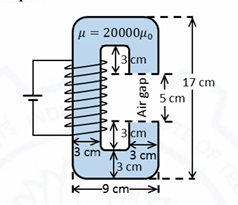
\includegraphics[width=0.4\textwidth]{figs/q63fig21.png}
\caption{Cross-section of an electromagnet.}
\label{fig:q53ph}
\end{figure}
Ignoring the fringe fields, the magnitude of the magnetic field $\vec{B}$ (in Tesla, rounded off to two decimal places) in the air-gap between the magnetic poles is \underline{\hspace{3cm}}.

\item The spin $\vec{S}$ and orbital angular momentum $\vec{L}$ of an atom precess about $\vec{J}$, the total angular momentum. $\vec{J}$ precesses about an axis fixed by a magnetic field $\vec{B_1} = 2B_0\hat{z}$, where $B_0$ is a constant. Now the magnetic field is changed to $\vec{B_2} = B_0(\hat{x}+\sqrt{2}\hat{y}+2\hat{z})$. Given the orbital angular momentum quantum number $l=2$ and spin quantum number $s=1/2$, $\theta$ is the angle between $\vec{B_1}$ and $\vec{J}$ for the largest possible values of total angular quantum number $j$ and its z-component $j_z$. The value of $\theta$ (in degree, rounded off to the nearest integer) is \underline{\hspace{3cm}}.
\hfill \textbf{(GATE PH 2021)}

\item The spin-orbit effect splits the $^{2}P \to {}^{2}S$ transition (wavelength, $\lambda=6521$ \text{Å}) in Lithium into two lines with separation of $\Delta\lambda = 0.14$ \text{Å}. The corresponding positive value of energy difference between the above two lines, in eV, is $m \times 10^{-5}$. The value of $m$ (rounded off to the nearest integer) is \underline{\hspace{3cm}}.
(Given: Planck's constant, $h = 4.125 \times 10^{-15}$ eV s \\
Speed of light, $c = 3 \times 10^8$ m s$^{-1}$)
\hfill \textbf{(GATE PH 2021)}

\begin{center}
\textbf{END OF THE QUESTION PAPER}
\end{center}

\end{enumerate}

\end{document}